\documentclass{article}
\usepackage{amsmath}
\usepackage{tikz}
\usetikzlibrary{arrows.meta}

\begin{document}

\begin{figure}[h]
    \centering
    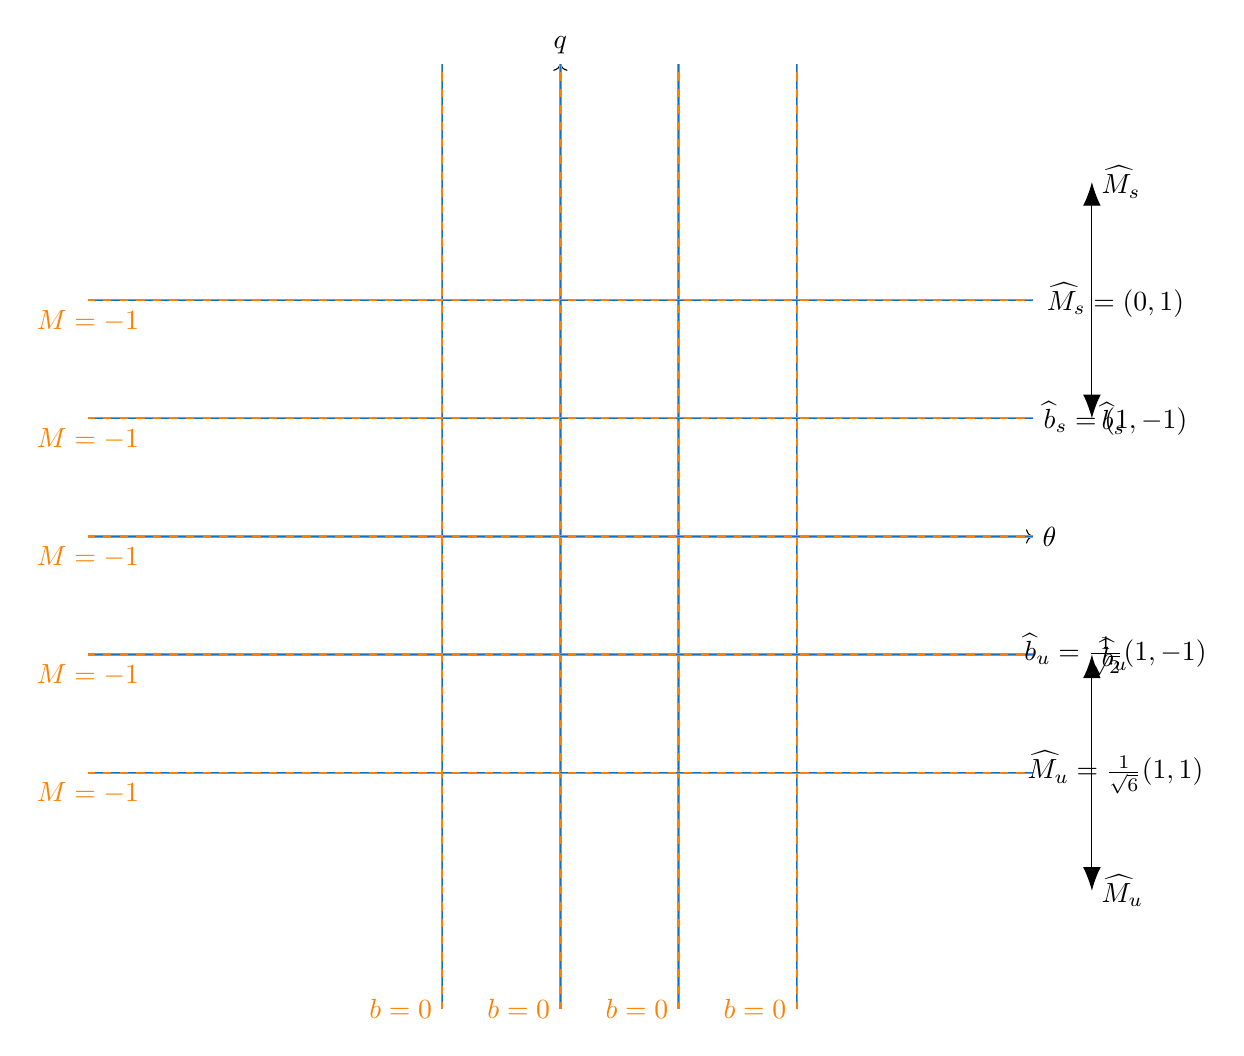
\begin{tikzpicture}[scale=1.5]
        % Axes
        \draw[->] (-4,0) -- (4,0) node[right] {$\theta$};
        \draw[->] (0,-4) -- (0,4) node[above] {$q$};

        % Lines
        \foreach \x/\y/\label in {-1/0/$b=-1$, 0/0/$b=0$, 1/0/$b=1$, 2/0/$b=2$}{
            \draw[orange, thick] (\x,4) -- (\x,-4) node[left] {$b=\y$};
            \draw[dashed, cyan!50!blue] (\x,4) -- (\x,-4);
        }
        \foreach \x/\y/\label in {-2/-1/$M=-2$, -1/-1/$M=-1$, 0/-1/$M=0$, 1/-1/$M=1$, 2/-1/$M=2$}{
            \draw[orange, thick] (4,\x) -- (-4,\x) node[below] {$M=\y$};
            \draw[dashed, cyan!50!blue] (4,\x) -- (-4,\x);
        }

        % Arrows
        \draw[-{Latex[length=3mm]}] (4.5,2) -- (4.5,3) node[right] {$\widehat{M}_s$};
        \draw[-{Latex[length=3mm]}] (4.5,2) -- (4.5,1) node[right] {$\widehat{b}_s$};
        \draw[-{Latex[length=3mm]}] (4.5,-2) -- (4.5,-3) node[right] {$\widehat{M}_u$};
        \draw[-{Latex[length=3mm]}] (4.5,-2) -- (4.5,-1) node[right] {$\widehat{b}_u$};

        % Labels for dual vectors
        \node at (4.7,2) {$\widehat{M}_s = (0,1)$};
        \node at (4.7,1) {$\widehat{b}_s = (1,-1)$};
        \node at (4.7,-2) {$\widehat{M}_u = \frac{1}{\sqrt{6}}(1,1)$};
        \node at (4.7,-1) {$\widehat{b}_u = \frac{1}{\sqrt{2}}(1,-1)$};
    \end{tikzpicture}
    \caption{
        The vectors $\left\{ \widehat{M}_s,\, \widehat{b}_s \right\}$ and $\left\{ \widehat{M}_u,\, \widehat{b}_u \right\}$ form orthonormal bases with respect to the inner products ${\langle \,\cdot\,,\,\cdot\, \rangle}_{s}$ and ${\langle \,\cdot\,,\,\cdot\, \rangle}_{u}$, respectively, as they were introduced in Definition \ref{def:pointwise_states_and_ips}, namely $\widehat{M}_s = (0,\,1)$, $\widehat{b}_s = (1,\,-1)$, $\widehat{M}_u = \frac{1}{\sqrt{6}} (1,\,1)$, and $\widehat{b}_u = \frac{1}{\sqrt{2}} (1,\,-1)$. Even though, especially in the saturated region $\left\{ q > 0 \right\}$, labelling these vectors with the moist variable $M$ and the buoyancy $b$ may at first appear perplexing, this is justified by the fact that their corresponding \emph{dual} vectors are precisely (multiples of) $M$ and $b$. Indeed: ${\langle \widehat{M}_s ,\, (\theta,\,q) \rangle}_{s} = \theta + q = M$, ${\langle \widehat{b}_s ,\, (\theta,\,q) \rangle}_{s} = \theta = b_s$, ${\langle \widehat{M}_u ,\, (\theta,\,q) \rangle}_{u} = \sqrt{\frac{3}{2}} (\theta + q) = \sqrt{\frac{3}{2}} M$, and ${\langle \widehat{b}_u ,\, (\theta,\,q) \rangle}_{u} = \frac{1}{\sqrt{2}} \theta - q = \frac{1}{\sqrt{2}} b_u$.
    }
    \label{fig:orthonormal_bases}
\end{figure}

\end{document}